\subsection{Design}
In designing the desktop user interface the first step was to identify the
main goals of our users, in order to make sure that the system delivered
the required information quickly and clearly. After a discussion it was 
agreed that the typical user would have two main priorities - checking 
whether a specific team had been elimated and viewing the league tables for
each division. This was further broken down into a list of functional requirements.

\begin{itemize}
\item Display eliminated teams.
\item Display all divisions/leagues.
\item Display all teams in a division.
\item Automatically update the display on startup.
\item Display certificate of elimination.
\end{itemize}

With these requirements in mind several paper prototypes were
created by different members of the team so as to increase the range of
ideas we could incorporate into the final design. These prototypes were
compared in terms of functional clarity and aesthetic appeal, with the 
effective elements of each taken and incorporated into a final prototype
design. This was the resulting wireframe.

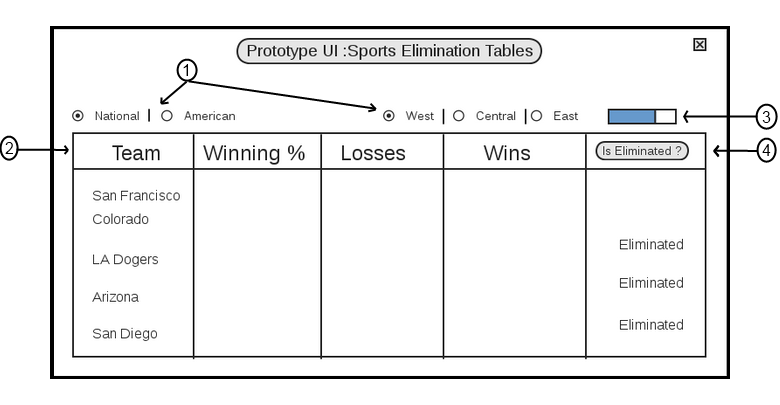
\includegraphics[width=\linewidth,keepaspectratio]
{images/Prototype_UI.png}

\begin{enumerate}
\item League navigation panel - allow the users to quickly and easily select the
league and division. Deliberately layed out and grouped left to right to indicate
that divisions are subsets of leagues.
\item Standings table - immediately display the currently selected divisions major 
statistics.
\item Loading bar - displays the progress of the Ford-Fulkerson algorithm.
\item Elimination indicator - indicate whether the team has been eliminated, both
trivially and non-trivially.
\end{enumerate}

This design focuses on serving the primary user needs by displaying the division 
rankings and elimination status on startup, which in the the best case scenario 
would mean the user would not need to input anything to get the desired information.

\subsection{Implementation}
The interface was written using the Java Swing framework - a popular toolkit used in
building graphical user interfaces for Java programs. The actual building of the interface
was a gradual and adaptive process, with the focus on getting a working version of the 
prototype up and running. This was accomplished and based on team feedback features were added
or removed. The completed Ford-Fulkerson algorithm ran almost instantly, rendering the loading 
bar unnecessary and so it was dropped. Date navigation buttons - including drop down date selectors -
were added to allow the user to move through the season chronologically. 

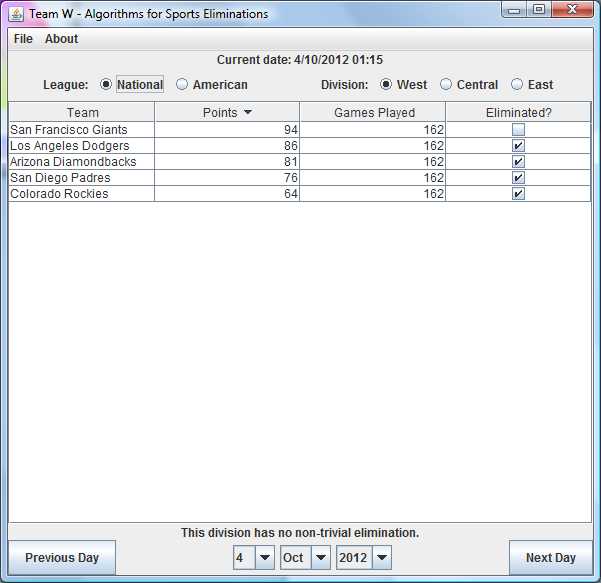
\includegraphics[width=\linewidth,keepaspectratio]
{images/finalDesktopUI.png}

This final version of the UI features three main components - a table with associated model, 
two sets of radio buttons and the date navigation panel, comprising of two buttons and three
drop down boxes. The work flow of the UI is similar for each of these components - they all 
have event listeners that set the data according to the user input and call a shared function 
(in order to minimise complexity). This update function gets the division chosen
by the user and plays the matches up to the current/selected date. It then updates the table 
model and redraws - now displaying the appropriate values, including the correct elimination status.
Additional features that were added after the base prototype was completed was a label
showing the current date to assist the date navigation and the ability
to display the certificate of elimination. Clicking on the is eliminated table cell will 
open a text box displaying the elimination details if they exist.